%!TEX root = main.tex

\documentclass[../main.tex]{subfiles}

\begin{document}

\appendix

\chapter{String Winding Measurement Photos}

\begin{figure}[h]
    \centering
    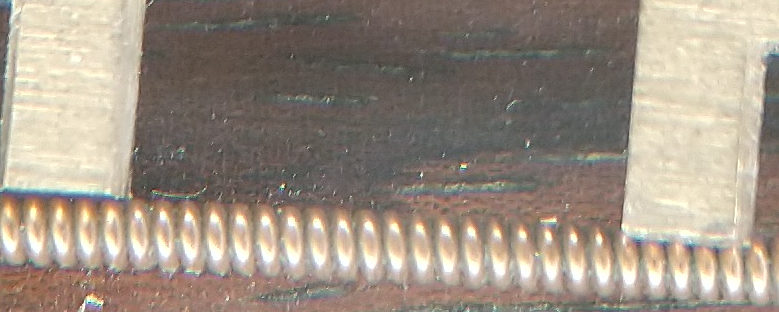
\includegraphics[scale=.45]{./images/pictures/WindingsEZoom.png}
    \caption{Photo of the low E string winding count for 1 cm}
    \label{fig:EStringWindings}
\end{figure}

\begin{figure}[h]
    \centering
    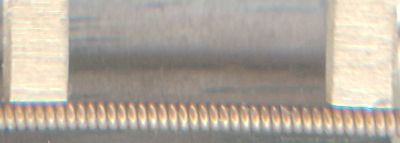
\includegraphics[scale=.45]{./images/pictures/WindingsAZoom.png}
    \caption{Photo of the A string winding count for 1 cm}
    \label{fig:AStringWindings}
\end{figure}

\begin{figure}[h]
    \centering
    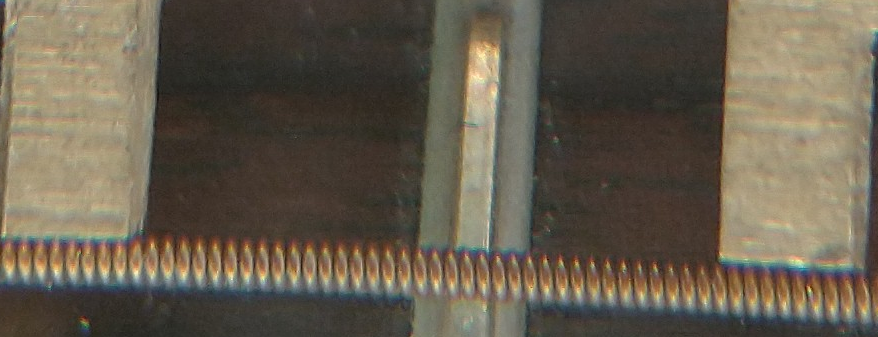
\includegraphics[scale=.5]{./images/pictures/WindingsDZoom.png}
    \caption{Photo of the D string winding count for 1 cm}
    \label{fig:DStringWindings}
\end{figure}

\chapter{Class Hierarchy}
Fill me in later

\chapter{Code and Sound Examples}
All the source code and sound examples can be found at the following GitHub repo:\\
\url{https://github.com/dgsmith1988/Masters-Thesis}

\end{document}